

%\newcommand*{\ACM}{}%

\ifdefined\ACM

%\documentclass[sigplan,screen]{acmart}
\documentclass[manuscript,screen,review]{acmart}

\else
 \documentclass[14pt]{article}
%\usepackage{libertine}
\usepackage{cuted}%\usepackage{widetext}
\input{./usepackage}
\usepackage{cancel}
\usepackage{subcaption}
\addbibresource{./sample.bib}

\fi

\begin{document}
\input{newcommands}
%\title{ $\textbf{QNC}_{1} \subset $ noisy-\textbf{BQP}}
\title{ Fault-Tolerainzing at Constant Depth Overhead }
\author{Michael Ben-Or \ \ David Ponarovsky}
\maketitle

\newcommand*{\Mbas}{\mathcal{X}^\prime}
\newcommand*{\bas}{\mathcal{X}}
\newcommand*{\sMbas}{\Mbas}
\newcommand*{\QQ}{C_{X}/C_{Z}^\perp }
\newcommand*{\trig}{ Triorthogonal }
\newcommand*{\Hyp}{ Hyperproduct }
\newcommand*{\Cin}{ C_{\text{initial}} }
\newcommand*{\Ctan}{ C_{\text{Tan}} }



\newcommand*{\QACze}{\mathbf{QAC}_{0}}
\newcommand*{\QNCzef}{\mathbf{QNC}_{0,f}}
\newcommand*{\QNCze}{\mathbf{QNC}_{0}}
\newcommand*{\QNCon}{\mathbf{QNC}_{1}}
\newcommand*{\NCon}{\mathbf{NC}_{1}}
\newcommand*{\noiseQNCon}{noisy-$\QNCon$}
\newcommand*{\QNC}{\mathbf{QNC}}
\newcommand*{\QNCG}{\mathbf{QNC_G}}
\newcommand*{\NC}{\mathbf{NC}}
\newcommand*{\QNCiG}{\mathbf{QNC_{G,i}}}


% Constant depth fault tolerance construction.   
\newcommand*{\CDO} {CDFT} 
%


\abstract{
  We study the overall depth overhead cost required for constructing fault-tolerant circuits. We focus on shallow depth circuit classes, in particular, $\QACze{}, \QNCzef{}$, $\QNCon{}$, and '$\QNC{}$ without reset gates', and certain known problem candidates for demonstrating quantum advantage such as factoring \cite{Shor_1997} and Instantaneous Quantum Polynomial-time \cite{Bremner_2017}, \cite{Paletta_2024}. We aim to answer whether there exists a fault tolerance with only constant overhead at the circuit's depth. A positive answer implies that computing logarithmic depth circuits when subjected to noise is not harder than computing in an ideal environment.

}

%
  \section{Introduction.} 
  
The Quantum Computation model is widely believed to be superior to classical models, offering asymptotic speedup in tasks such as factoring \cite{Shor_1997}, searching \cite{grover1996fast}, simulating, and more relative to the best-known classical solutions. Yet even though there is almost complete agreement about the superiority of the ideal quantum model, there is still a debate over whether it is possible to implement complex computation in the real world, where the qubits and gates are subject to faults. Similarly, the feasibility of realizing classical computation has also been an open question, In fact the question about the feasibility of computation under noise is almost as ancient as the computer science field itself, initialized by Von Neumann \cite{Neumann+1956+43+98} at the time that classical computation putted in debuts. Time been pass and the followed works had pointed that not even a polynomial computation in the presence of noise is still reasonable but one can implement a fault tolerance version at a most constant times cost at the circuits depth \cite{Pippenger}. Or in asymptotic sense, classical computation in the presence of noise is as exactly hard as computation in ideal environment.  

Recently, the feasibility question has been raised again, this time regarding quantum computing, and while an intensive work has been done, and also succeed to prove that polynomial quantum computation can be made fault tolerance, \cite{aharonov1999faulttolerant},\cite{gottesman2014faulttolerant} and even with only constant overhead at the original circuit width \cite{grospellier:tel-03364419}, the required depth over-head is still not well understood. We stress out that in all the familiar constructions, in construct to Pippenger \cite{Pippenger}, original constant-depth gates are mapped to asymptotically grow\footnote{Note, that here, classical computation is also counted in the overall depth cost} depth gates. 


Moreover, even the depth overhead is particularly interesting as today's quantum machines are challenged to maintain quantum states for a long time. The limitations of these machines have motivated research to define NISQ, which stands for Noisy Intermediate-Scale Quantum, referring to the current era of quantum computing characterized by quantum processors that have a limited number of qubits and are prone to errors due to noise. In addition to NISQ, another common characterization for limited quantum computation is computation without reset gates, which has been proved to be impossible when restricted to polynomial space \cite{aharonov1996limitationsnoisyreversiblecomputation}. Having a constant depth-overhead fault tolerance scheme would imply the feasibility of log depth computation in that model.
  
%This work address the above, We ask whether a magnitude depth overhead is an unavoidable price that one has to pay. And, in particular, whether an ideal $\QNCon$, the class of problem can be decided by logarithmic depth quntum circuits, can be computed in noisy-$\QNCon$ circuits. We show how using the ideas presented in \cite{grospellier:tel-03364419} and \cite{Pippenger} gives almost immediately $\QNCzef \subset$ \noiseQNCon and that sampling from IQP, Instantaneous Quantum Polynomial-time \cite{Bremner_2017}, \cite{Paletta_2024}, also can be done in logarithmic depth circuits.    
This work addresses the above. We ask whether a magnitude depth overhead is an unavoidable price that one has to pay, If a Constant Depth Fault Tolerance Construction (\CDO{}) exists, and if so, how to construct it. In particular, whether an ideal $\QNCon{}$, the class of problems that can be decided by logarithmic depth quantum circuits, can be computed in noisy-$\QNCon{}$ circuits.

Additionally, we extend the question beyond the standard classes and ask about fault-tolerant sampling. Specifically, we consider several sampling processes by shallow quantum circuits, which are believed to be infeasible for classical circuits, such as Instantaneous Quantum Polynomial-time \cite{Bremner_2017}, \cite{Paletta_2024}, and ask about the depth efficiency of their fault-tolerant version.

%$\QNCzef \subset$ \noiseQNCon 
%
%We show how using the ideas presented in \cite{grospellier:tel-03364419} and \cite{Pippenger} gives almost immediately $\QNCzef \subset$ \noiseQNCon and that sampling from IQP, , also can be done in logarithmic depth circuits.



  
  
The proposal is organized as follows. \Cref{sec:nota} presents the notations, formal definitions, and states the open problems that will be studied through the research. Then, \Cref{sec:opt} describes strategies to prove \CDO{}. In particular, it lists primitives that can be used to achieve it and discusses how far we are from obtaining them. Having said that, \Cref{sec:passi} presents the first cues against the possibility of \CDO{} and provides the entry points to prove the impossibility claim. Finally, \Cref{sec:app} discusses the applications and implications of either the correctness of \CDO{} or the impossibility of \CDO{}, from both theoretical and practical views.

%\input{notations.tex}

\section{Local Decoders}

\begin{definition}
  Light cone,
\end{definition}

\begin{definition} 
    We say that $D$ is a local decoder if when applied against $2p(1-p)$-depolarized channel: 
    \begin{itemize}
      \item  There exists function $M : (0,1) \rightarrow (0,1) $ such that the probability of each bit being flipped is $M(2p(1-p)) < p^{\frac{100}{99}}$.
      \item There is a constant $l$ such that for any bit, there are only $(\Delta)^{l}$ bits on which the event of it being flipped depends.
    \end{itemize}
For example, if we take $k$ large enough and consider the $(n,k)$-Toric, then both the swift-rule and the flip upon majority are local decoders.
\end{definition}


  \begin{definition}
Consider the moment after the application of the depolarizing channel, and right before the correction by the decoder.

For a subset of qubits $S$, we say that a qubit $x \in S$ is depended if there exists $y \in S$ such:
\begin{enumerate}
  \item Either $x$ and $y$ share a check that is not satisfied. (Type I)  
  \item Or, $x$ and $y$ have checks which share a bit that was flipped by the application of the channel. (Type II)
\end{enumerate}
  \end{definition}


  
  \textbf{Dependence Type I}
  \begin{figure}[h]
    \begin{tikzpicture}[scale=0.7]
      %\draw node at (1.5,4.5) {$v_{2}$ is flipped.};

\draw node (u1) at (3,3) [draw,shape=rectangle]{$u_1$};
\draw node (x) at (0,6) [draw,shape=circle]{$x$};
\draw node (y) at (0,0) [draw,shape=circle]{$y$};
\draw (u1) -- (y)
  (u1) -- (x);
\end{tikzpicture}
  \end{figure}

  \begin{align*}
    & \prb{ (x,y) \in e | u_{1} \text{ is satisfied} }  \\
    & = \prb{ x \in e | u_{1} \text{ is satisfied}  }  \prb{ y \in e | u_{1} \text{ is satisfied}  } \\ 
    & \le \prb{ x \in e }\prb{ y \in e }
  \end{align*}


  \textbf{Dependence Type II}
  \begin{figure}[h]
    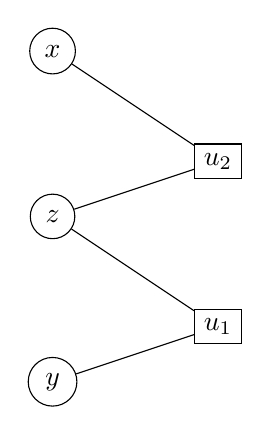
\begin{tikzpicture}[scale=0.7]
      %\draw node at (1.5,4.5) {$v_{2}$ is flipped.};

\draw node (u1) at (3,1) [draw,shape=rectangle]{$u_1$};
\draw node(u2) at (3,4) [draw,shape=rectangle]{$u_2$};
\draw node (x) at (0,6) [draw,shape=circle]{$x$};
\draw node (z) at (0,3) [draw,shape=circle]{$z$};
\draw node (y) at (0,0) [draw,shape=circle]{$y$};
\draw (u1) -- (y)
  (u1) -- (z)
  (u2) -- (x)
  (u2) -- (z);
\end{tikzpicture}
  \end{figure}

  \begin{align*}
    & \prb{ (x,y) \in e | z \text{ is not flipped} }  \\
    & = \prb{ x \in e | z \text{ is not flipped} }  \prb{ y \in e | z \text{ is not flipped} } \\ 
    & \le \prb{ x \in e }\prb{ y \in e }
  \end{align*}






\section{Memory}


\begin{definition} 
    Let $\rho^{(0)}$ be a mixed state over codewords. Define:

    \begin{equation*}
        \rho^{(t)} =  D \circ \mathcal{N} \rho^{(t-1)} 
    \end{equation*}
\end{definition}

  \begin{theorem} There is $p_{\text{th}} \in (0,1)$ such that for any $p < p_{\text{th}}$ and any bounded Hermitian operator $X$ we have: 
    \begin{equation*}
      \Tr X\rho^{(t)} \le \Tr X  \mathcal{N}_{p} \left( \rho \right)  + t||X|| e^{- \Theta( \sqrt{n}) }
    \end{equation*}
\end{theorem}

\begin{lemma} There exists a constant $c >0 $, such:
    \begin{equation*}
      \Tr X  D \circ \mathcal{N}_{p} \circ \mathcal{N}_{p} \left( \rho \right)  \le \Tr X  \mathcal{N}_{p} \left( \rho \right)  + 2||X|| e^{- \Theta( \sqrt{n}) }
    \end{equation*}
\end{lemma}

\begin{proof}
  By induction on $t$.
  \begin{align*}
    \Tr X\rho^{(t)}  &=  \Tr X D \circ \mathcal{N}_{p} \rho^{(t-1)} \\
      & \le   \Tr X D \circ  \mathcal{N}_{p} \circ \mathcal{N}_{p} \left( \rho \right)  + (t-1)||X|| e^{- \Theta( \sqrt{n}) } \\
      & \le \Tr X  \mathcal{N}_{p} \left( \rho \right)  + t||X|| e^{- \Theta( \sqrt{n}) }
  \end{align*}
  When in the last transition we used the lemma. 
\end{proof}








\printbibliography
\end{document}


